\documentclass[12pt, a4paper]{article}

\usepackage[utf8]{inputenc}
\usepackage[russian]{babel}
\parindent 0pt
\parskip 8pt
\usepackage{amsmath}
\usepackage{amssymb}
\usepackage{array}
\usepackage[left=2.3cm, right=2.3cm, top=2.7cm, bottom=2.7cm, bindingoffset=0cm]{geometry} % headheight=0pt,
\usepackage{hyperref}
\usepackage{graphicx}
\usepackage{multicol}
\usepackage{fancyhdr} 
\usepackage{extramarks}
\usepackage[usenames,dvipsnames]{color}
\usepackage{titlesec}
\usepackage{tikz}
\definecolor{grey}{RGB}{128,128,128}

\pagestyle{fancy}
\fancyhf{}
\lhead{Билет № 1.5}
\chead{Протоколы когерентности кэш-памяти}
\rhead{\thepage}
\lfoot{made with Ы}
\cfoot{}
\rfoot{\today}
\renewcommand\headrulewidth{0.4pt}
\renewcommand\footrulewidth{0.4pt}

\titlespacing*{\section}{0pt}{5pt}{0pt}
\titlespacing*{\subsection}{0pt}{5pt}{0pt}
\titlespacing*{\subsubsection}{0pt}{5pt}{0pt}

\begin{document}
\section{Зачем оно надо?}
Представим, что у нас есть два процессора CPU0 и CPU1. CPU0 считал строку X. Теперь она есть в CPU0\_Cache. CPU1 считал строку X. Теперь она есть в CPU1\_Cache. CPU0 пишет в строку X новое значение и возвращает в память. CPU1 снова считывает строку X и получает старое закэшированное значение. Очень жаль.\\
Чтобы такого не происходило, придумали протоколы и механизмы когерентности.
\section{Механизмы когерентности}
Два самых известных механизма когерентности это \textit{snooping} и использование \textit{директорий}(directory-based), у каждого из них есть преимущества и недостатки.
\subsection{Snooping}
Каждый запрос передается (\textit{broadcast}) всем другим узлам.\\
Протоколы, базирующиеся на этом механизме, быстрее, если у шины достаточная пропускная способность, т.к. все запросы/ответы видны всем процессорам. Недостаток в том, что такие системы плохо масштабируются. Каждый запрос должен передаваться всем узлам сети, а это значит, что вся система становится больше, ширина шины и ее пропускная способность тоже должны увеличиваться.
\subsection{Использование директорий*}
При таком механизме, общие данные хранятся в специальной общей директории, которая и решает проблему когерентности: при запросе на чтение процессор должен спросить разрешение у директории на то, чтобы загрузить данные из памяти себе в кэш. Если процессор изменяет кэш-линию, то директория либо обновляет данные других кэшей, либо говорит им выкинуть свои копии.
Директории медленнее, но не нуждаются в широкой шине, т.к. сообщения передаются от одного узла к другому, а не всем узлам сети. По этой причине многие многопроцессорные системы (>64 CPU) используют именно этот механизм.
\section{Протоколы когерентности кэш-памяти}
\subsection{MSI}
\subsubsection{Описание}
\begin{itemize}
    \item \textbf{M}odified - кэш-линия была изменена, т.е данные в кэше не совпадают с данными в памяти. Кэш несет ответственность за запись такой линии в память.
    \item \textbf{S}hared - кэш-линия не изменен и присутствует в read-only состоянии хотя бы в одном кэше. Кэш может выкинуть такую линию без записи в память.
    \item \textbf{I}nvalid - кэш-линия или не присутствует в данном кэше, или была аннулирована запросом шины.
\end{itemize}
\textbf{Запрос на чтение}\\
В CPU0\_Cache пришел запрос на чтение кэш-линия X.
\begin{itemize}
    \item Если X Modified или Shared, CPU0\_Cache возвращает кэш-линия X, и всё хорошо.
    \item Если же X Invalid, то CPU0\_Cache должен выяснить, не находится ли эта линия где-то в другом кэше в состоянии Modified.
    \begin{itemize}
        \item Если в CPUN\_Cache линия X находится в состоянии Modified, он должен записать эту кэш-линию в память и перевести её в состояние Shared или Invalid. После этого CPU0\_Cache считывает кэш-линию X из памяти или у кэша, у которого блок в состоянии Shared.
        \item Если в CPUN\_Cache кэш-линия X находится в состоянии Shared, CPU0\_Cache получает кэш-линию от CPUN\_Cache.
        \item Если ни в одном другом кэше нет линии X, кэш обращается к памяти.
    \end{itemize}
\end{itemize}
После операции чтения кэш-линия X в CPU0\_Cache находится в состоянии Shared.\\
\textbf{Запрос на запись}
В CPU0\_Cache пришел запрос на запись в кэш-линию X.
\begin{itemize}
    \item Если кэш-линия в состоянии Modified, кэш изменяет её локально и всё у него хорошо.
    \item Если кэш-линия в состоянии Shared, то кэш говорит всем остальным выкинуть свои копии. Далее данные могут быть изменены локально.
    \item Если кэш-линия в состоянии Invalid, то кэш должен сообщить всем остальным кэшам выкинуть свои копии. Если в каком-то из кэшей линия в состоянии Modified, то этот кэш может как записать кэш-линию в память, так и передать её CPU0\_Cache. Это зависит от реализации. Если на этот момент CPU0\_Cache еще не получил кэш-линию X, он запрашивает её у памяти.
\end{itemize}
После операции записи кэш-линия X в CPU0\_Cache находится в состоянии Modified\\
\begin{figure}[h]
    \centering
    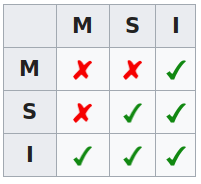
\includegraphics[scale=0.7]{./images/MSI.png}
    \caption{Разрешенные состояния кэш-линии X}
    \label{fig:MSI}
\end{figure}
\subsubsection{Проблемы?}
Да, чаще всего у процессора какие-то свои данные, которые есть только у него. Тем не менее, каждый раз, когда ему надо сделать запись в Shared, он держит в курсе остальных, что надо бы эти данные выкинуть. Шина забивается мусорными сообщениями.
\section{MESI}
\subsection{Что нового?}
Добавили еще одно состояние, теперь:
\begin{itemize}
    \item \textbf{S}hared - кэш-линия содержится \textit{больше}, чем в одном кэше.
    \item \textbf{E}xclusive - кэш-линия содержится \textit{только} в одном кэше и не изменена.
\end{itemize}
\begin{figure}[h]
    \centering
    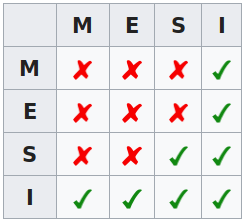
\includegraphics[scale=0.7]{./images/MESI.png}
    \caption{Разрешенные состояния кэш-линии X}
    \label{fig:MESI}
\end{figure}
\subsection{Есть проблемы?}
Да, когда несколько процессоров пишут в одну и ту же кэш-линию, ее постоянно приходится сбрасывать в память.
А еще когда процессор запрашивает линию, которая в нескольких других находится в состоянии Shared, то отвечают все и забивают шину.
\section{MOESI}
Это вариация \testbf{AMD} на тему MESI.
\subsection{Что изменилось?}
Добавили еще одно состояние, теперь:
\begin{itemize}
    \item \textbf{O}wned - этот кэш один из нескольких, у кого есть копия этой кэш-линии, но только он может вносить изменения. Состояние Owned позволяет делиться измененными кэш-линиями, не записывая изменения в память. Кэш-линия может быть переведена в состояние Modified, после того, как все остальные кэши выкинут свои копии, и в состояние Shared, после записи изменений в память.
    \item \textbf{S}hared - эта кэш-линия - одна из нескольких копий в системе. Кэш не может вносить изменения в эту кэш-линию. Линия может как совпадать с памятью (ни у одного кэша нет этой линии в состоянии Owned), так и быть измененной (где-то есть кэш, у которого эта кэш-линия Owned). Кэш-линия может быть переведена в состояние Modified или Exclusive, после того, как остальные кэши выкинут свои копии.
\end{itemize}
\begin{figure}[h]
    \centering
    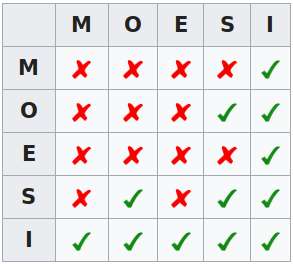
\includegraphics[scale=0.6]{./images/MOESI.png}
    \caption{Разрешенные состояния кэш-линии X}
    \label{fig:MOESI}
\end{figure}
\subsection{Преимущества}
Из-за того, что не можем не писать измененные данные в память, получаем выигрыш по скорости, если шина от кэша до процессора сильно жирнее и быстрее, чем от кэша до памяти.
\subsection{Недостатки}
Не можем быстро читать чистые (неизмененные) линии. Если у каких-то двух кэшей есть линия в состоянии Shared, и она не изменена, то третий скорее получит эту линию от памяти, чем от кэшей.
\section{MESIF}
Вариация \textbf{Intel} на тему MESI
\subsection{Что нового?}
\begin{itemize}
    \item \textbf{F}orward - специальный вид состояния Shared, показывает, что кэш должен отвечать на запросы шины по этой кэш-линии.
\end{itemize}
\subsection{Преимущества}
Не загружаем шину ответами кэшей.
\section{MOESIF}
Можно сделать. Но никто не сделал.
\end{document}